\section{Evaluation}\label{sec:eval}
The proposed framework is temporarily evaluated in terms of its ability to model users' preferences solely based on text labels of garments regardless of the photos. The following subsections would separately describe our evaluation approaches and results.

\subsection{Experiment Settings}
At first we acquired the garment information from Taobao where one set of garment consists several pictures and a text label describing the garment. By this way we have got 1772 garments in total as our raw data. The next step is to convert the chromatic pictures into scalable gray-scale pictures by OpenCV. After this step the preprocessing is done. 
 
The next thing we need is to acquire the users' preferences, and fortunately we successfully invited 24 volunteers to assess the garments and rate them. Meanwhile we set up a website and record every volunteer's scoring, and as a consequent we got approximately 60 ratings per volunteer summing up to 1553 ratings in total.

When considering the text labels, we manually chose 322 keywords as text features and Figure \ref{fig:freq} shows the frequency of each feature label. In the $Y$ axis are the frequencies, i.e. how many times a feature label appears in the set of text descriptions of rated garments, while the $X$ axis are the IDs of each feature label.

Temporarily we only focused on text label part, and ignore the pictures. And as for the selection of learning machines, we finally chose LIBSVM \cite{CC01a} as the tool to perform SVM learning.

\begin{figure}
  \centering
  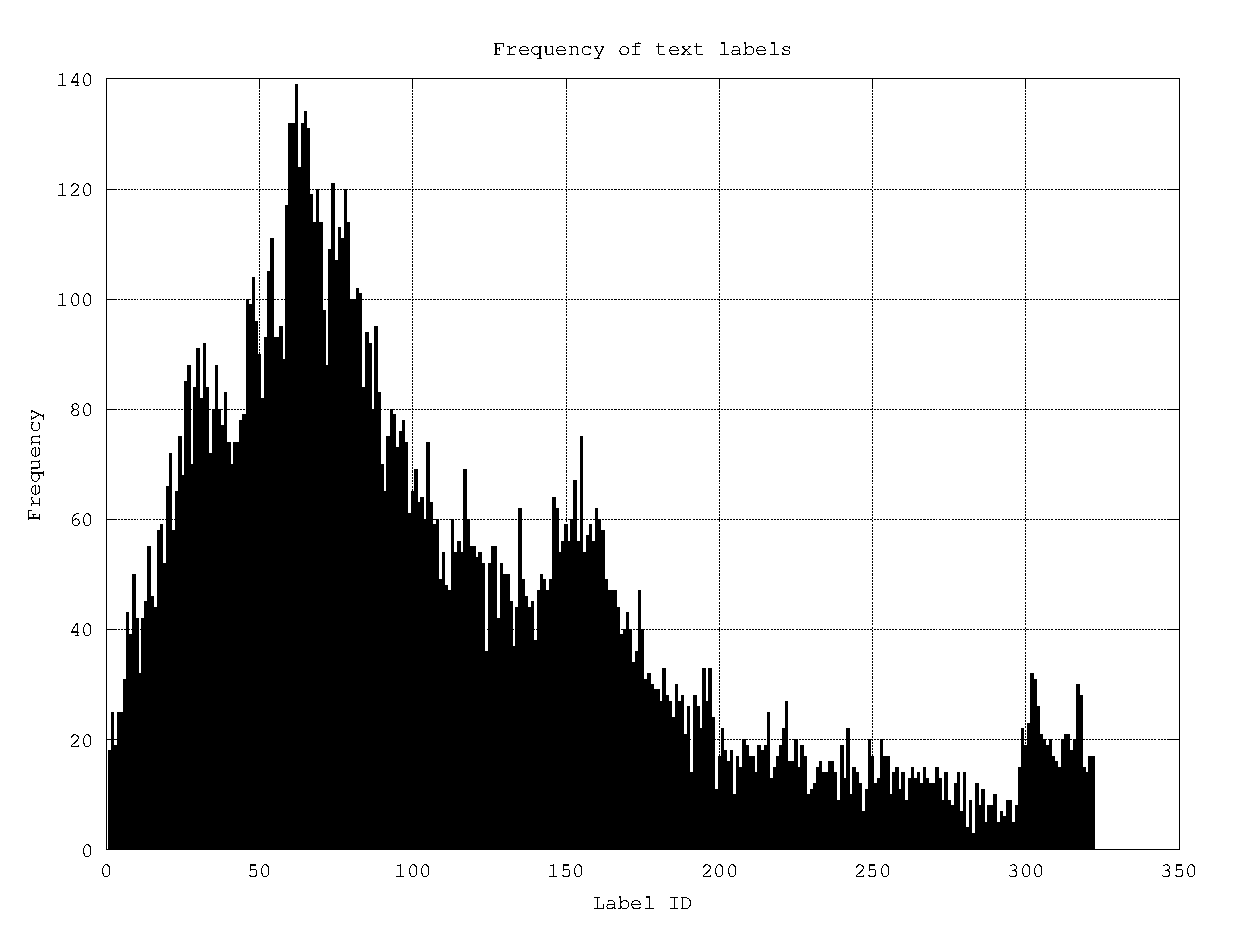
\includegraphics[width=0.9\textwidth]{frequency}
  \caption{Text label frequency}
  \label{fig:freq}
\end{figure}

\subsection{Website}

The section describes the website we set up for collecting user preferences.

Figure \ref{fig:website} shows the screenshots of the website.
Figure \ref{fig:website1} is a synthesized screenshot of both \emph{user rating} (top right) and \emph{product recommending} (middle right) user interface. The top left part shows the images of the product. When the user moves the mouse pointer over the image, a larger image will be shown in the top right part, as shown in \ref{fig:website2}. The bottom part of the page shows the textual descriptions of the product.

\begin{figure}[htb]
  \centering
  \subfigure[Synthesized screenshot of both \emph{user rating} and \emph{product recommending} user interface]{
    \label{fig:website1}
    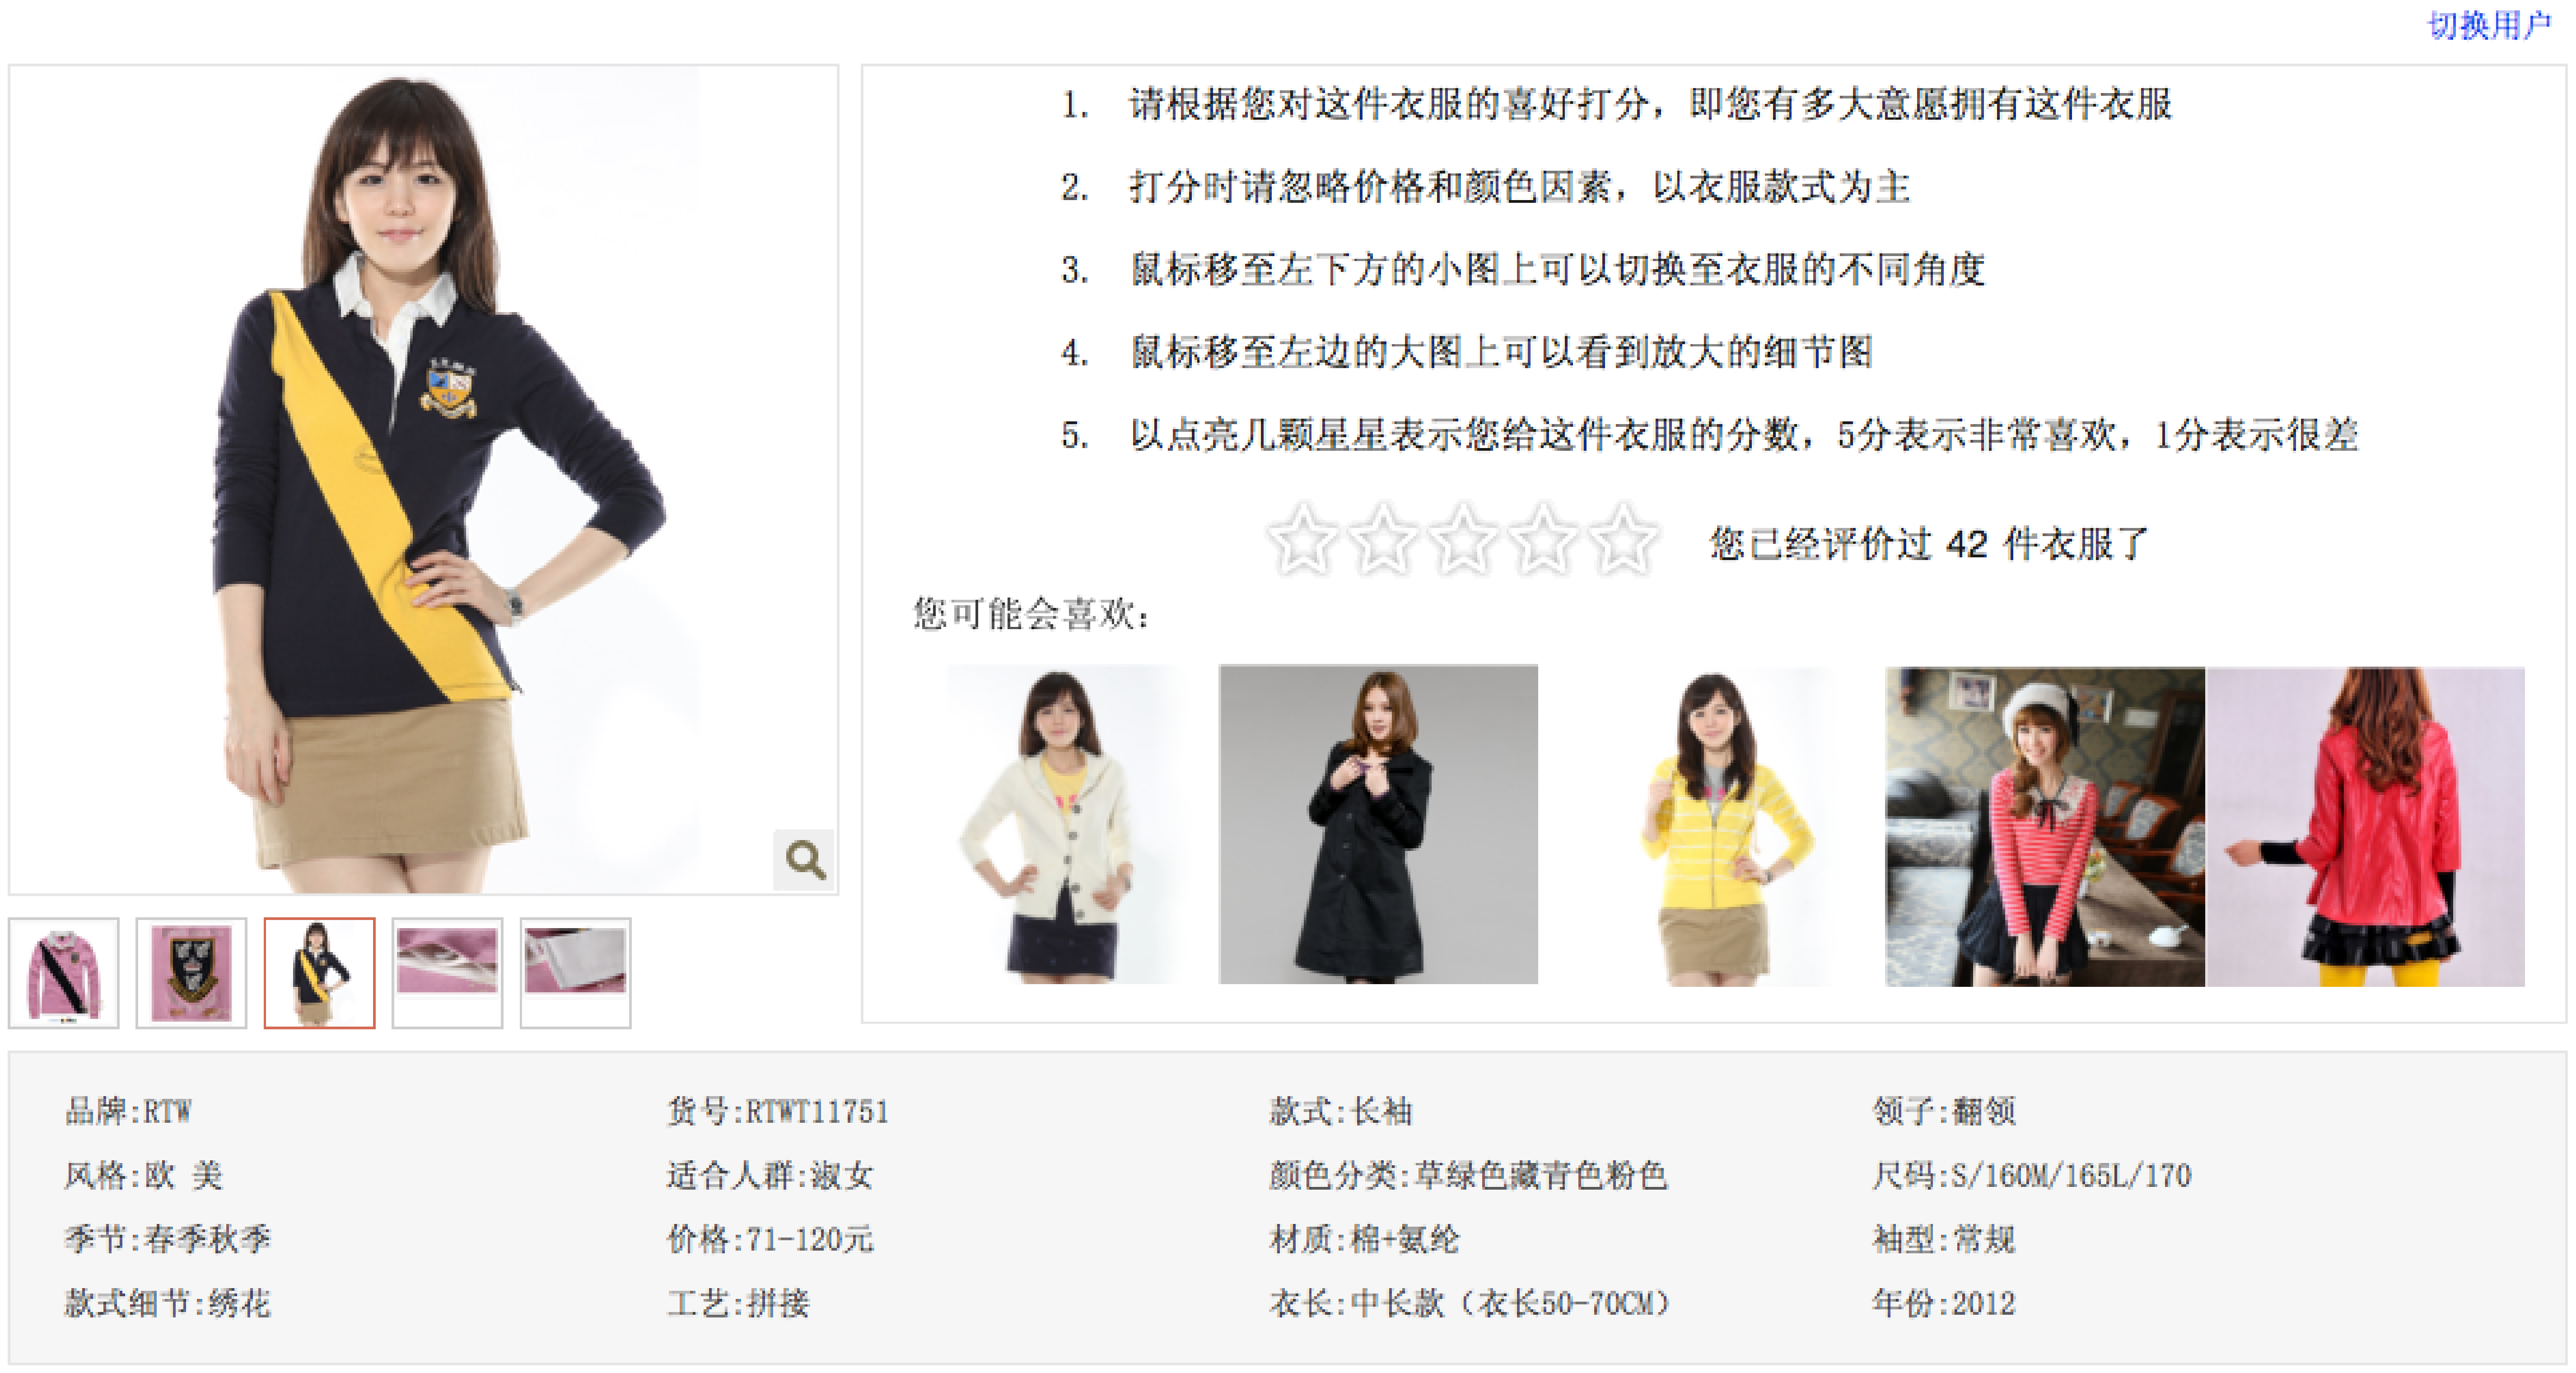
\includegraphics[width=0.8\textwidth]{website1}}
  \qquad
  \subfigure[Screenshot of viewing details of a product image]{
    \label{fig:website2}
    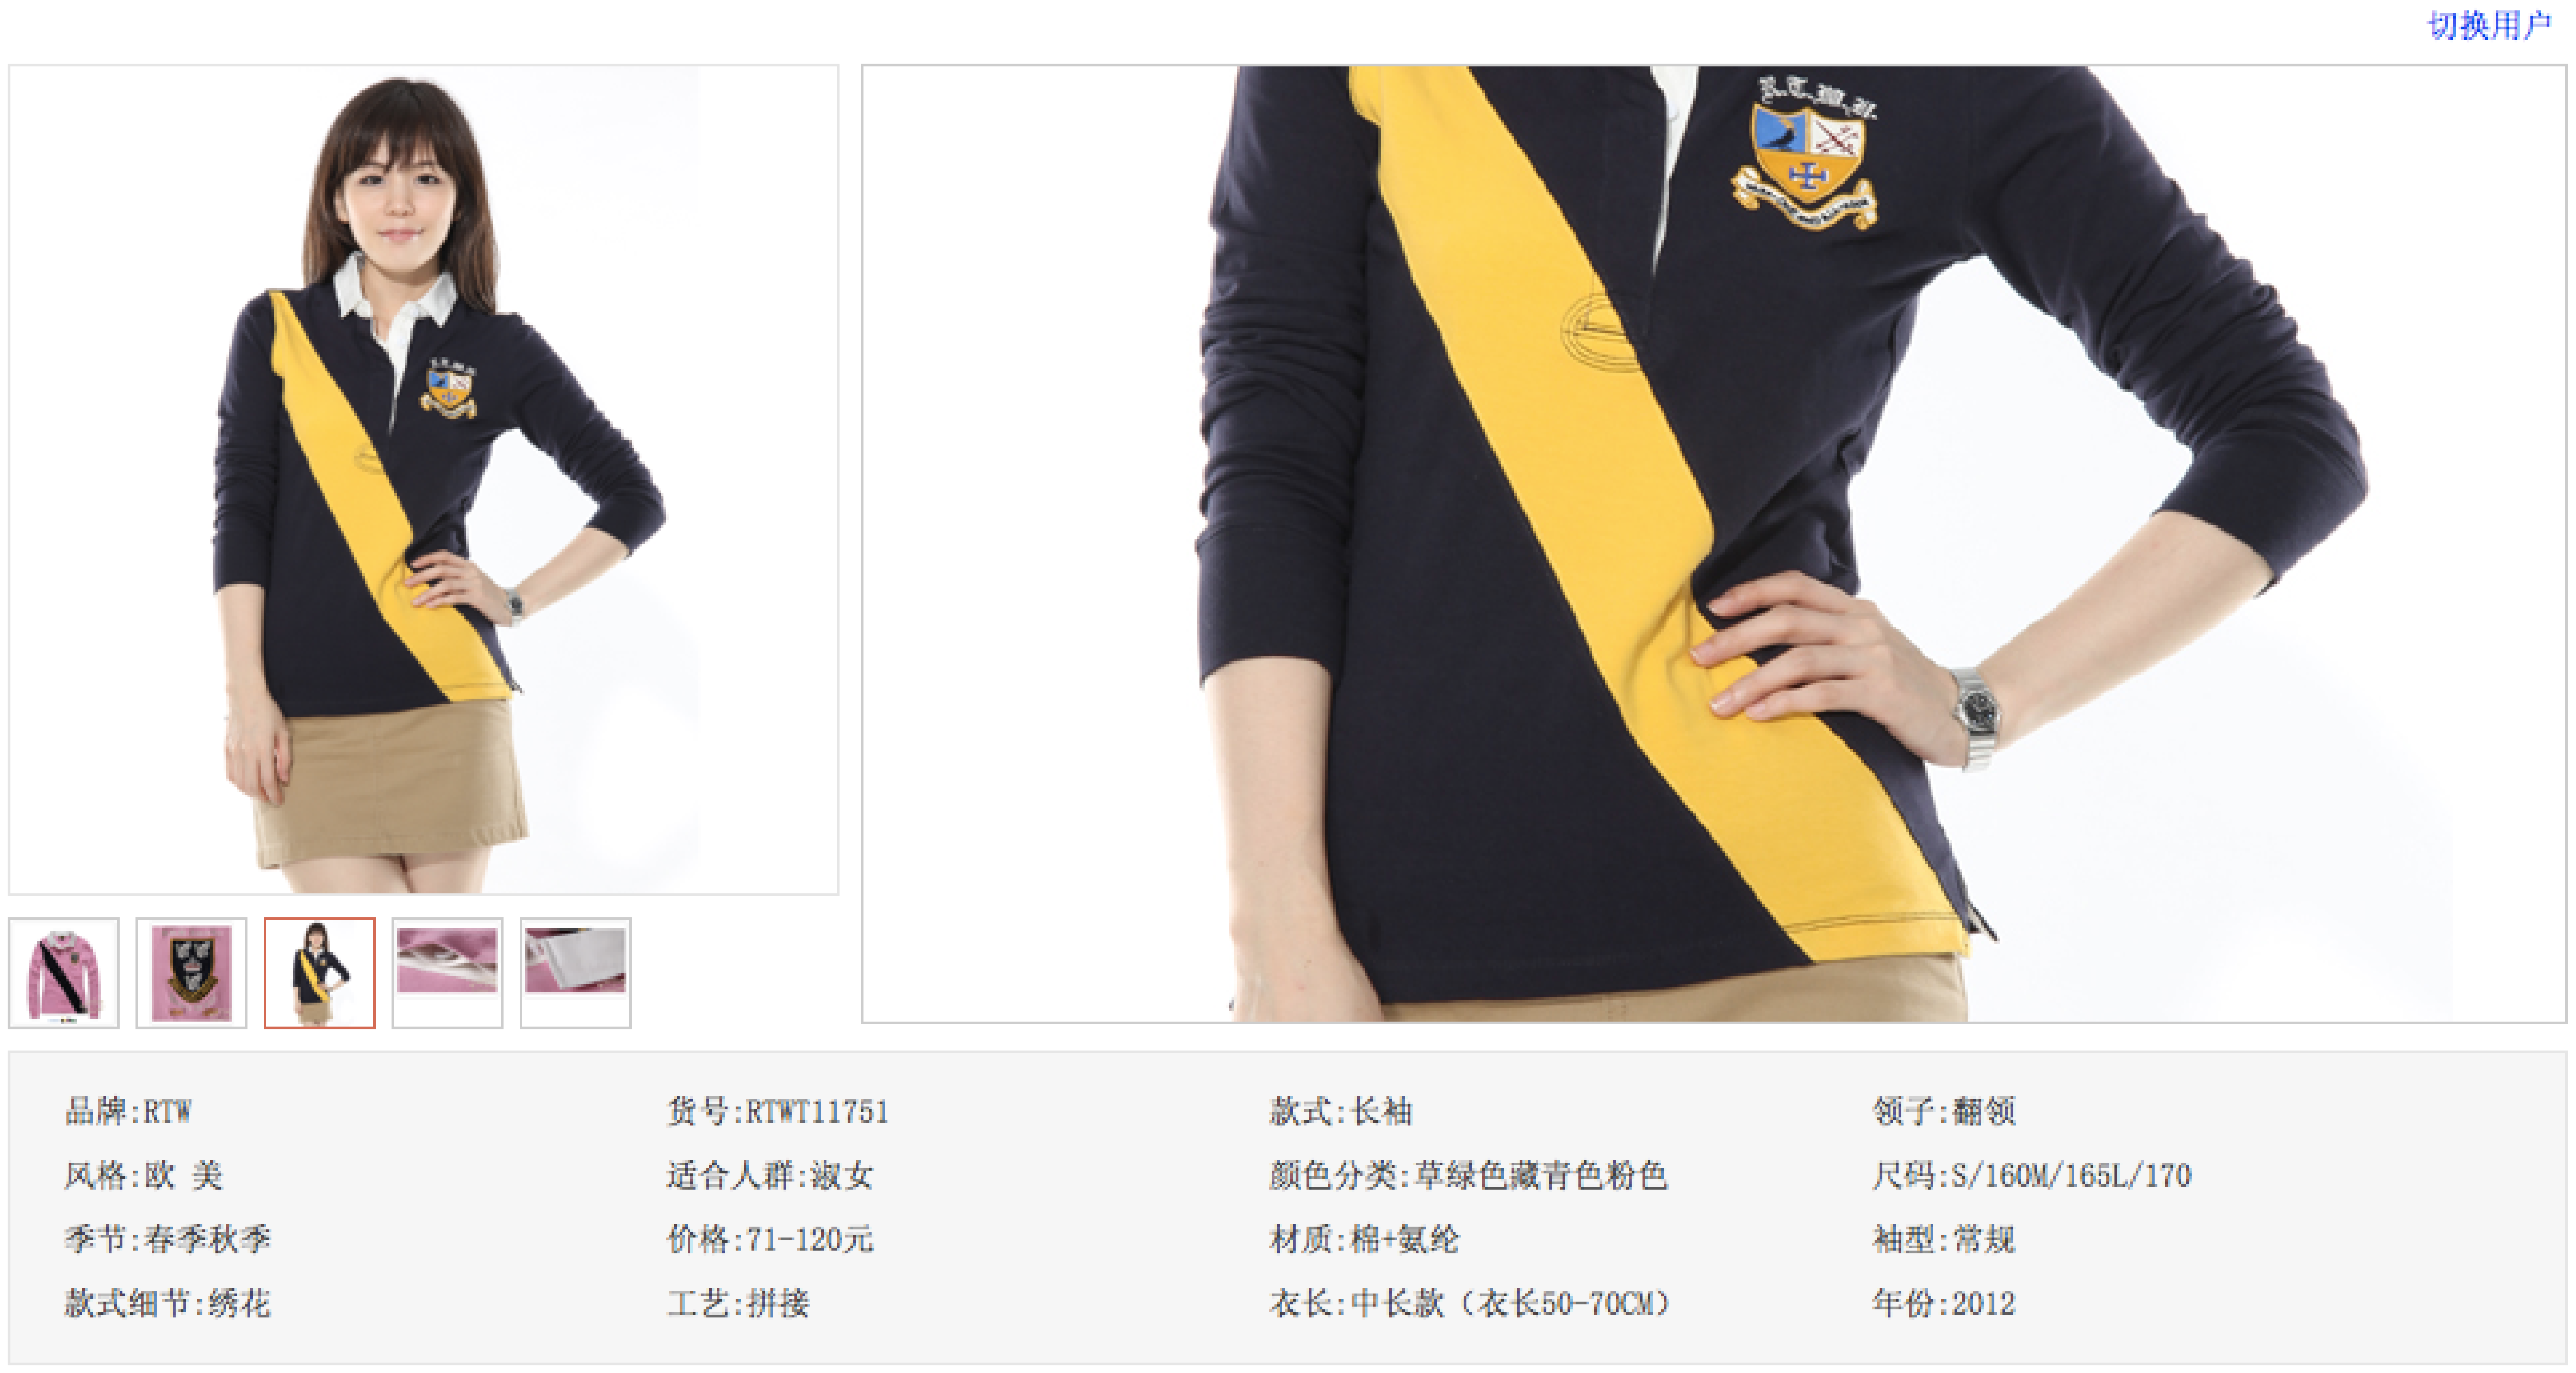
\includegraphics[width=0.8\textwidth]{website2}}
  \caption{Screenshots of our website for collecting user preferences}
  \label{fig:website}
\end{figure}

The website is written in PHP and deployed on Linux with Apache HTTP server. It randomly displays unrated products to the current user, collects user ratings of the products, and stores the ratings to a relational database for further investigation. The source code is available at \url{https://github.com/stfairy/recsys-website}.


\subsection{Results and Interpretation}
After acquiring the necessary data as input of the SVM, we began our training and assessing. Since we focused on every volunteer's individuality and personal preferences, we performed  the learning process to every one. 
Table 1 shows the results of LIBSVM learning after parameter modification, with the accuracy of 5-fold cross-validation.It implies that even with text features alone the accuracies could be high enough to make recommendations. However it is worth noticing that over-fitting is prone to occur since the learning set we use are extremely small. It is expected that after combining graphical features this potential problem could be alleviated. 

\begin{table}
  \centering  % used for centering table
  \begin{tabular}{c c | c c} % centered columns (2 columns)
    \hline                        %inserts double horizontal lines
    UserID & Accuracy & UserID & Accuracy \\ [0.9ex] % inserts table 
    %heading
    \hline                  % inserts single horizontal line
    1 & 89.0511\% & 13 & 94.1176\% \\
    2 & 92.5373\% & 14 & 89.3939\% \\
    3 & 80.9122\% & 15 & 93.7500\% \\
    4 & 88.4615\% & 16 & 96.6667\% \\
    5 & 91.3462\% & 17 & 93.3333\% \\
    6 & 90.0000\% & 18 & 94.5946\% \\
    7 & 86.8852\% & 19 & 85.7143\% \\
    8 & 89.4737\% & 20 & 89.4231\% \\
    9 & 97.0588\% & 21 & 88.3721\% \\
    10 & 78.3019\% & 22 & 89.7059\% \\
    11 & 82.0755\% & 23 & 90.4762\% \\
    12 & 85.0000\% & 24 & 95.1613\% \\[1ex]  
    \hline %inserts single line
  \end{tabular}
  \caption{LIBSVM 5-fold cross-validation accuracies} % title of Table
  \label{table:nonlin} % is used to refer this table in the text
\end{table}
